\documentclass[14pt]{beamer} %Makes presentation
%\documentclass[handout]{beamer} %Makes Handouts
\usetheme{Singapore} %Gray with fade at top
\useoutertheme[subsection=false]{miniframes} %Supppress subsection in header
\useinnertheme{rectangles} %Itemize/Enumerate boxes
\usecolortheme{seagull} %Color theme
\usecolortheme{rose} %Inner color theme

\definecolor{light-gray}{gray}{0.75}
\definecolor{dark-gray}{gray}{0.55}
\setbeamercolor{item}{fg=light-gray}
\setbeamercolor{enumerate item}{fg=dark-gray}

\setbeamertemplate{navigation symbols}{}
%\setbeamertemplate{mini frames}[default]
\setbeamercovered{dynamics}
\setbeamerfont*{title}{size=\Large,series=\bfseries}

%\setbeameroption{notes on second screen} %Dual-Screen Notes
%\setbeameroption{show only notes} %Notes Output

\setbeamertemplate{frametitle}{\vspace{.5em}\bfseries\insertframetitle}
\newcommand{\heading}[1]{\noindent \textbf{#1}\\ \vspace{1em}}

\usepackage{bbding,color,multirow,times,ccaption,tabularx,graphicx,verbatim,booktabs,fixltx2e}
\usepackage{colortbl} %Table overlays
\usepackage[english]{babel}
\usepackage[latin1]{inputenc}
\usepackage[T1]{fontenc}
\usepackage{lmodern}

%\author[]{Thomas J. Leeper}
\institute[]{
  \inst{}%
  Department of Government\\London School of Economics and Political Science
}


\title{Description and Evidence Gathering}



\date[]{}

\begin{document}

\frame{\titlepage}

\frame{\tableofcontents}

\section{Review Quantitative Description}
\frame{\tableofcontents[currentsection]}

\frame{

\frametitle{Last Week's Material}

\begin{itemize}\itemsep0.5em
\item Data Description
\item Variable summaries
	\begin{itemize}
	\item Statistics
	\item Tabulation
	\item Aggregation
	\end{itemize}
\item Visualization
\end{itemize}

}

% challenges? questions?


\frame{

\frametitle{Preview}


\begin{itemize}\itemsep0.5em
\item You have everything you need to complete:
	\begin{itemize}
	\item Problem set 1
	\item Problem set 2
	\end{itemize}
\item<2-> Next week is reading week, so no lecture or class
\item<3-> Keep thinking about what kinds of topics interest you as possible research proposals
\end{itemize}

}



\section{Observation and Description}
\frame{\tableofcontents[currentsection]}


\frame{

\frametitle{{\large Features of \textit{Quantitative} Description}}

\begin{itemize}\itemsep0.25em
\item A \textit{rectangular} dataset (case-by-variable)
\item A clear \textit{unit of analysis}
\item Typically multiple cases
\item Quantitative and qualitative measures
\item Calculation of summary \textit{statistics}
\item Inferences based on ``dataset observations''
\end{itemize}

}

\frame{

\frametitle{{\large Dataset Observation (DSO)}}

``\textbf<4>{a score} for \textbf<2>{a case} on \textbf<3>{a variable}''

\begin{center}
\begin{tabular}{lrrr}
State & Year & \textbf<3>{Var1} & Var2 \\
\textbf<2>{Afghanistan} & \textbf<2>{2016} & \textbf<2->{1} & \textbf<2>{TRUE} \\ 
Afghanistan & 2015 & \textbf<3>{1} & TRUE \\
Algeria & 2016 & \textbf<3>{1} & FALSE \\
Algeria & 2015 & \textbf<3>{0} & TRUE \\
\dots \\
\end{tabular}
\end{center}

}

\frame{

\frametitle{Description Beyond DSOs}

\begin{itemize}\itemsep0.5em
\item Sometimes hear about ``qualitative'' and ``quantitative'' research
\item This divide is illusory because all research is qualitative and some involves quantitative description
\item Role of quantitative analysis
	\begin{itemize}
	\item The primary research objective
	\item A piece of evidence that is analyzed together with other descriptions
	\end{itemize}
\end{itemize}

}

\frame{}


% cases



\frame{

\frametitle{{\large Goals of Descriptive Research}}

\begin{enumerate}\itemsep1em
\item To \textit{answer} research questions
\item To \textit{generate} research questions
\item<2-> To do both of these, \textit{iteratively}
\end{enumerate}

}


\frame{

\frametitle{{\large Ex.: Galileo's Drawings of Sunspots}}

\vspace{1em}

\href{http://galileo.rice.edu/sci/observations/ssm_slow.mpg}{\includegraphics[width=\textwidth]{images/sunspotspanel.png}}

\vspace{2em}

{\tiny
Source: Public Domain, \href{http://earthobservatory.nasa.gov/Features/SolarMax/}{NASA}
}
}



\frame{

\frametitle{Ex.: Broad Street Cholera}

\begin{itemize}\itemsep0.5em
\item 1854 outbreak of cholera in London
	\begin{itemize}
	\item Around Broad Street (Soho)
	\item 616 eventual deaths
	\end{itemize}
\item<2-> Causal RQ: What causes transmission of cholera?
\item<3-> Descriptive RQ: Who exactly is contracting cholera?
\end{itemize}

}

\frame{

\begin{center}
\only<1>{\includegraphics[height=.98\textheight]{images/broadstreet}}
\only<2>{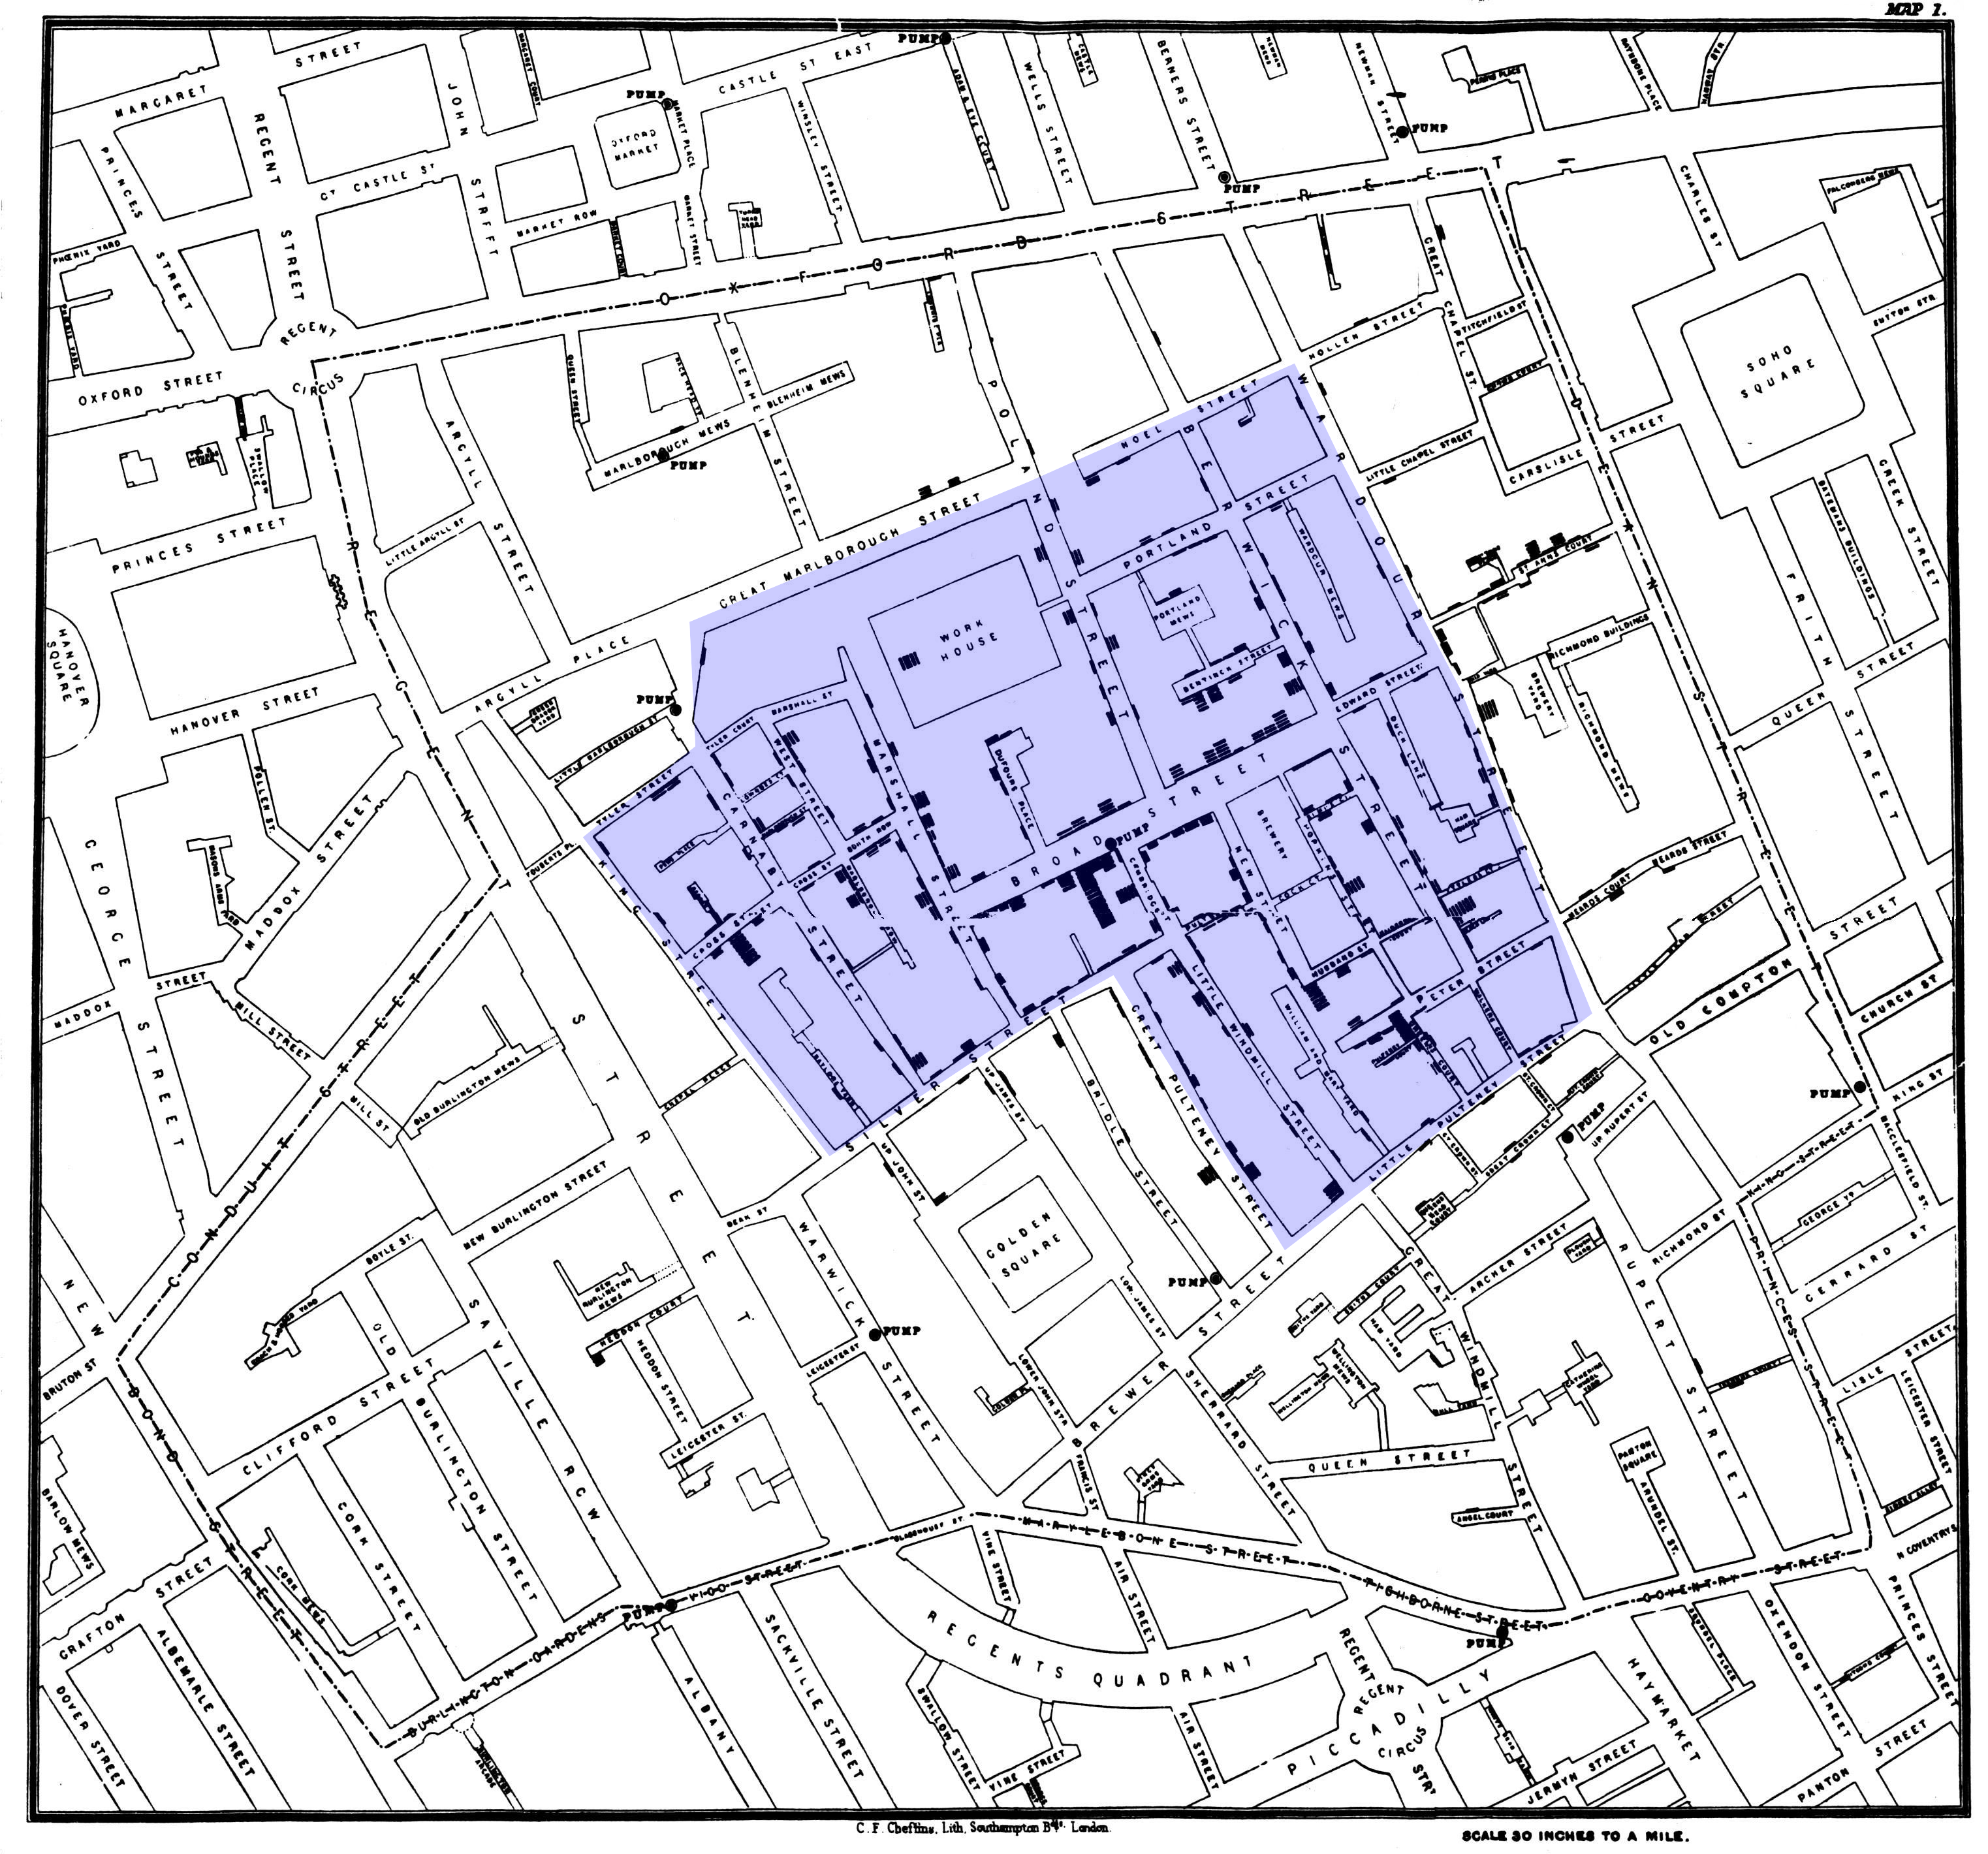
\includegraphics[height=.98\textheight]{images/broadstreet-1}}
\only<3>{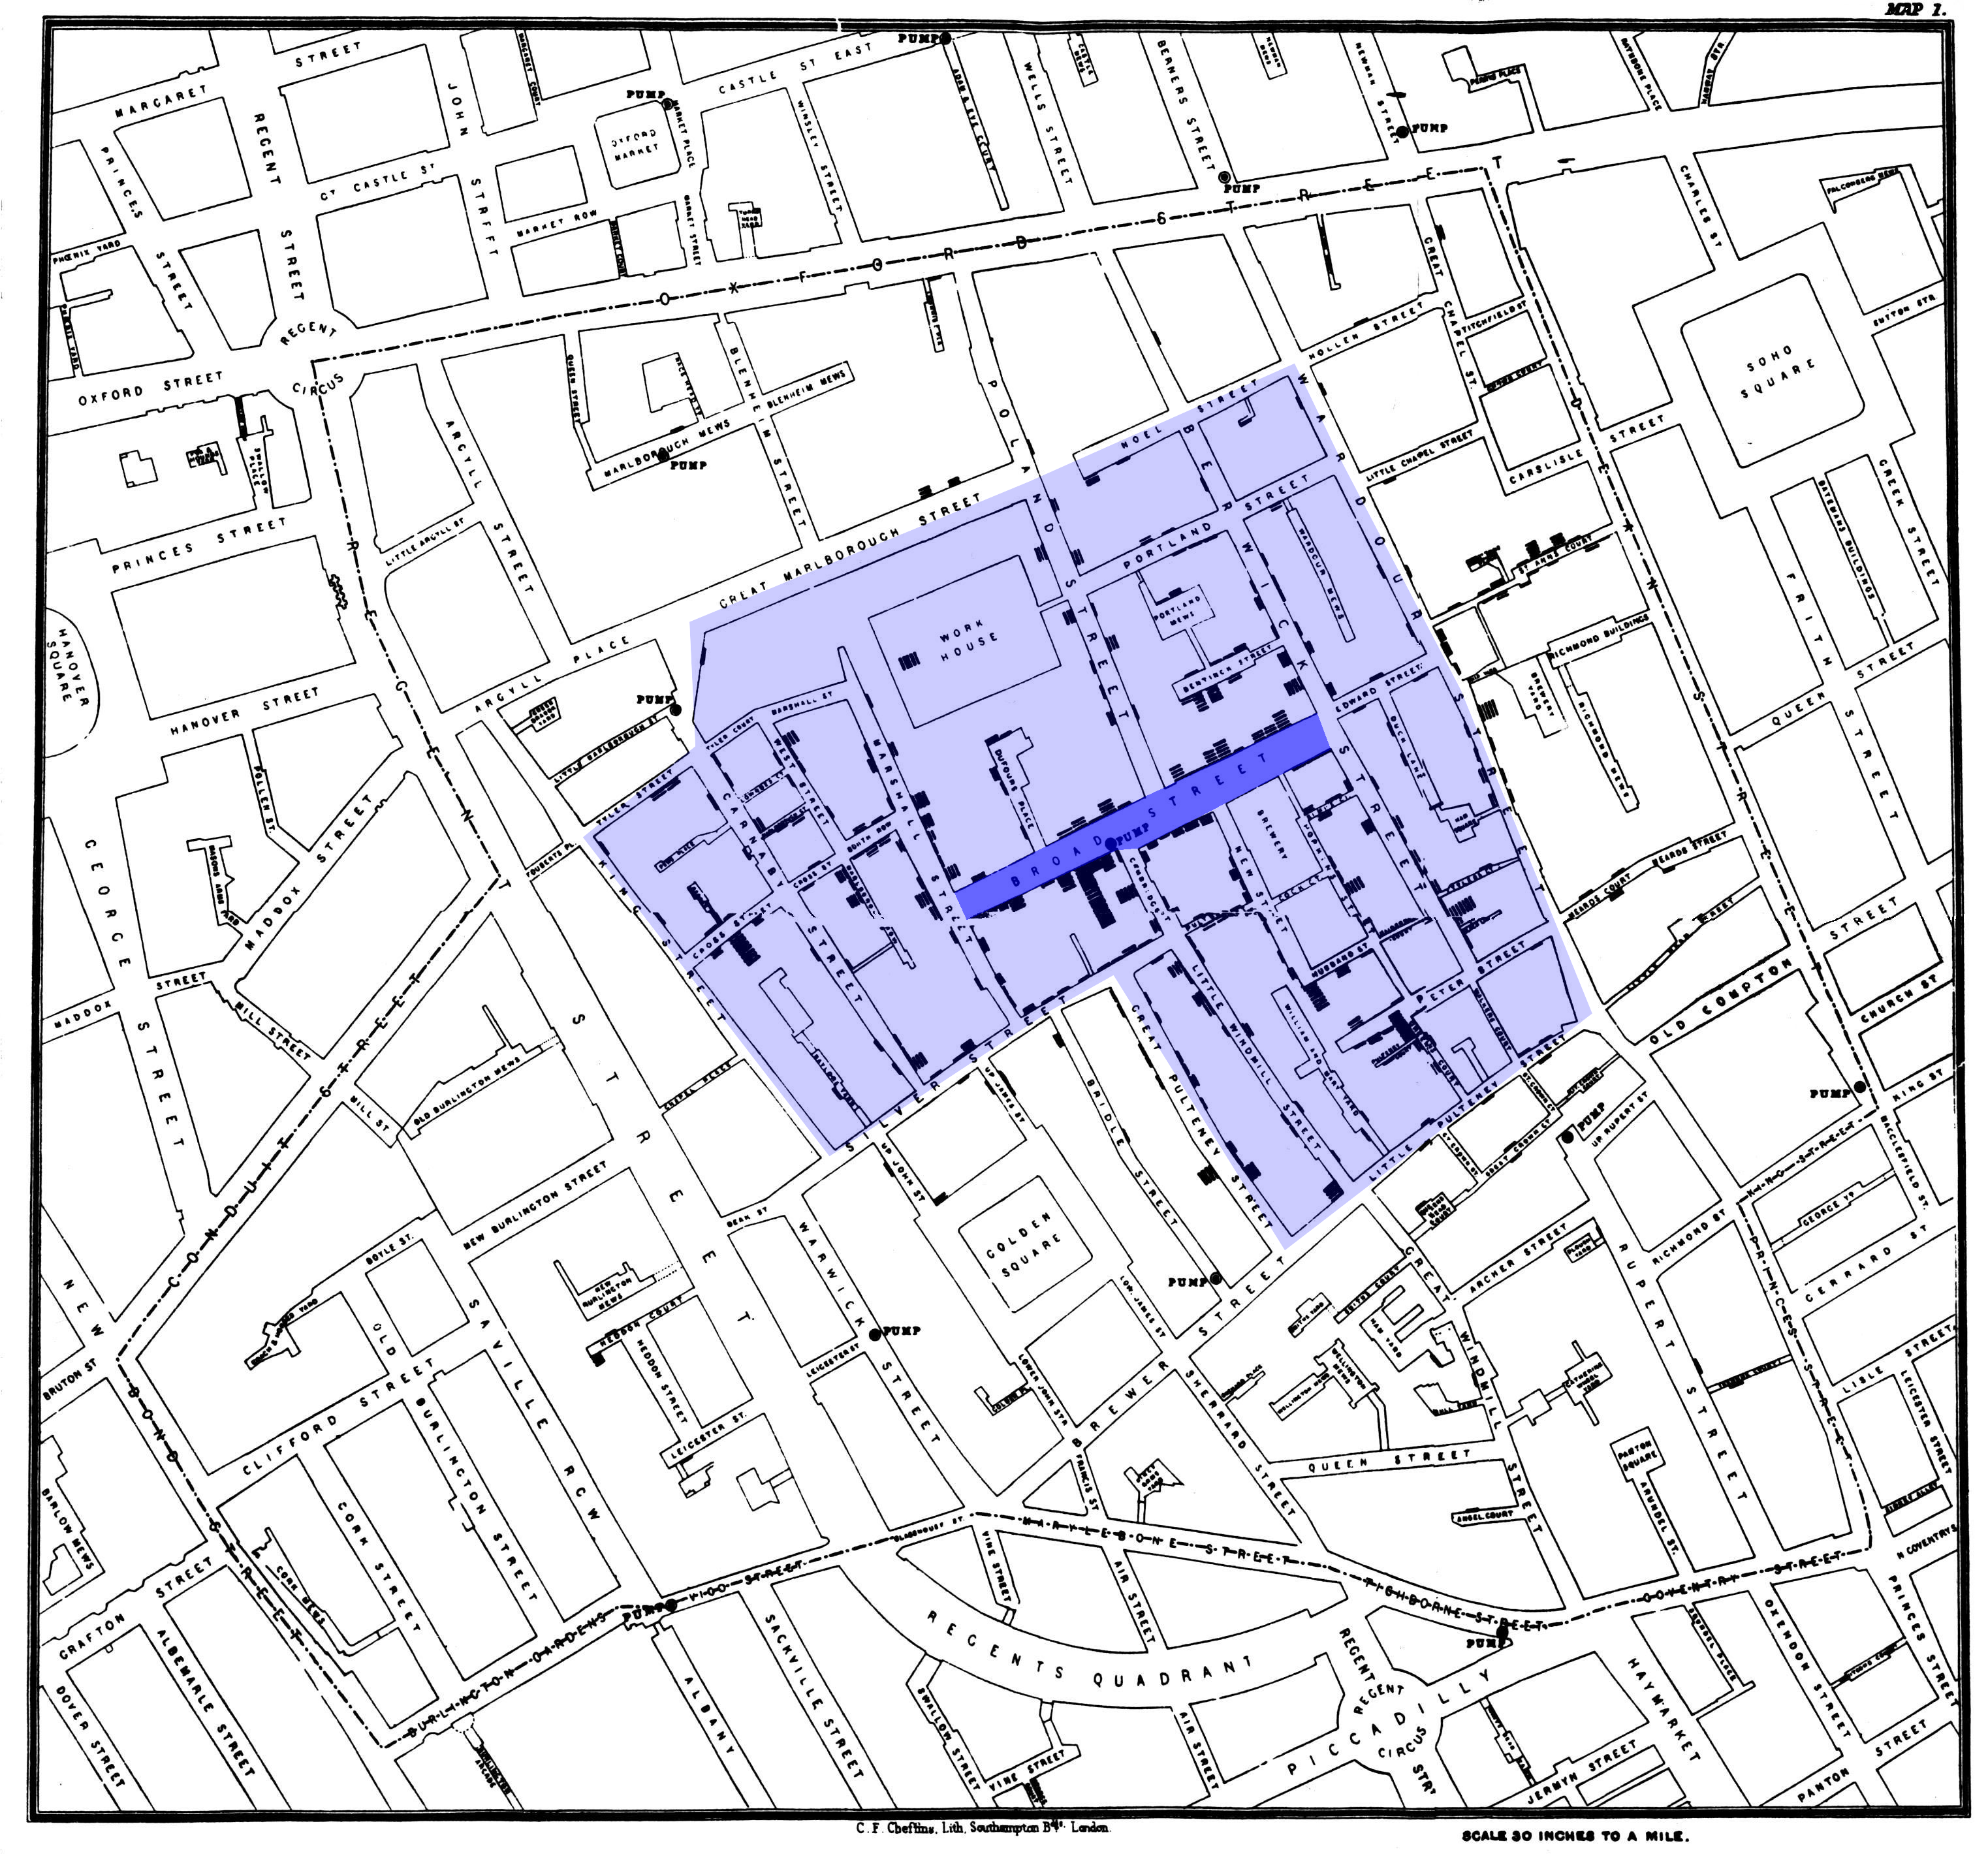
\includegraphics[height=.98\textheight]{images/broadstreet-2}}
\only<4>{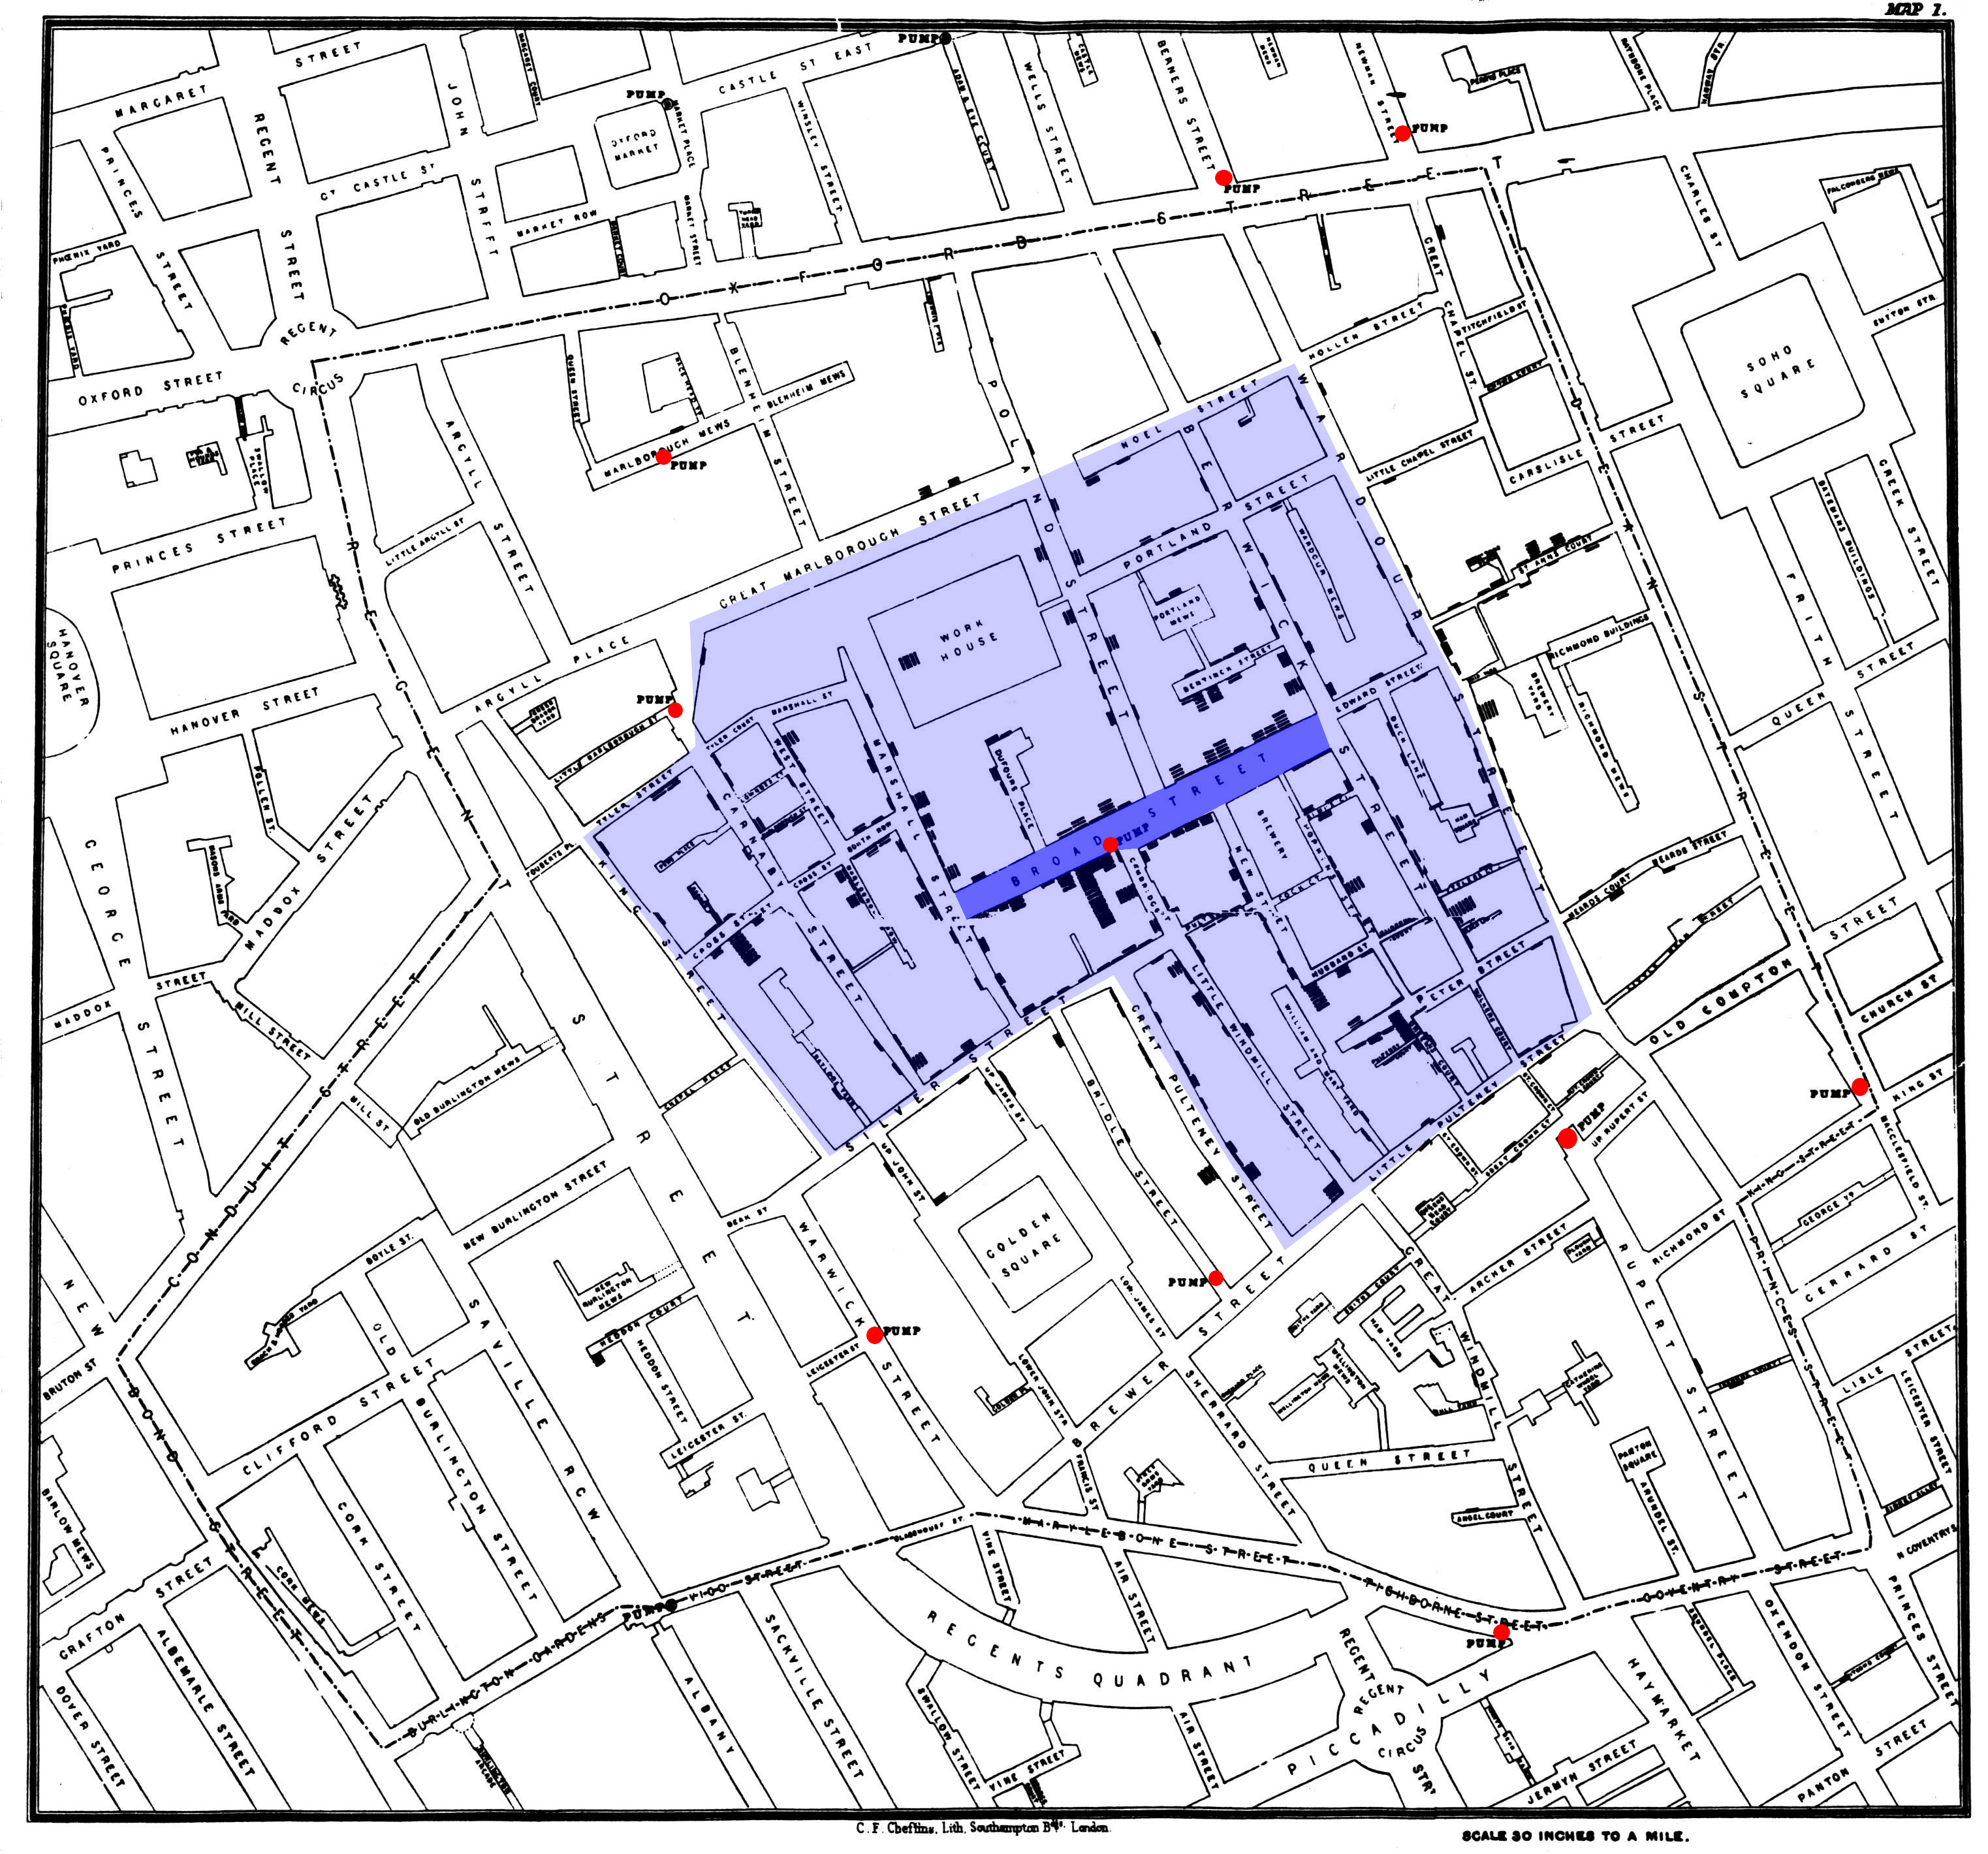
\includegraphics[height=.98\textheight]{images/broadstreet-3}}
\only<5>{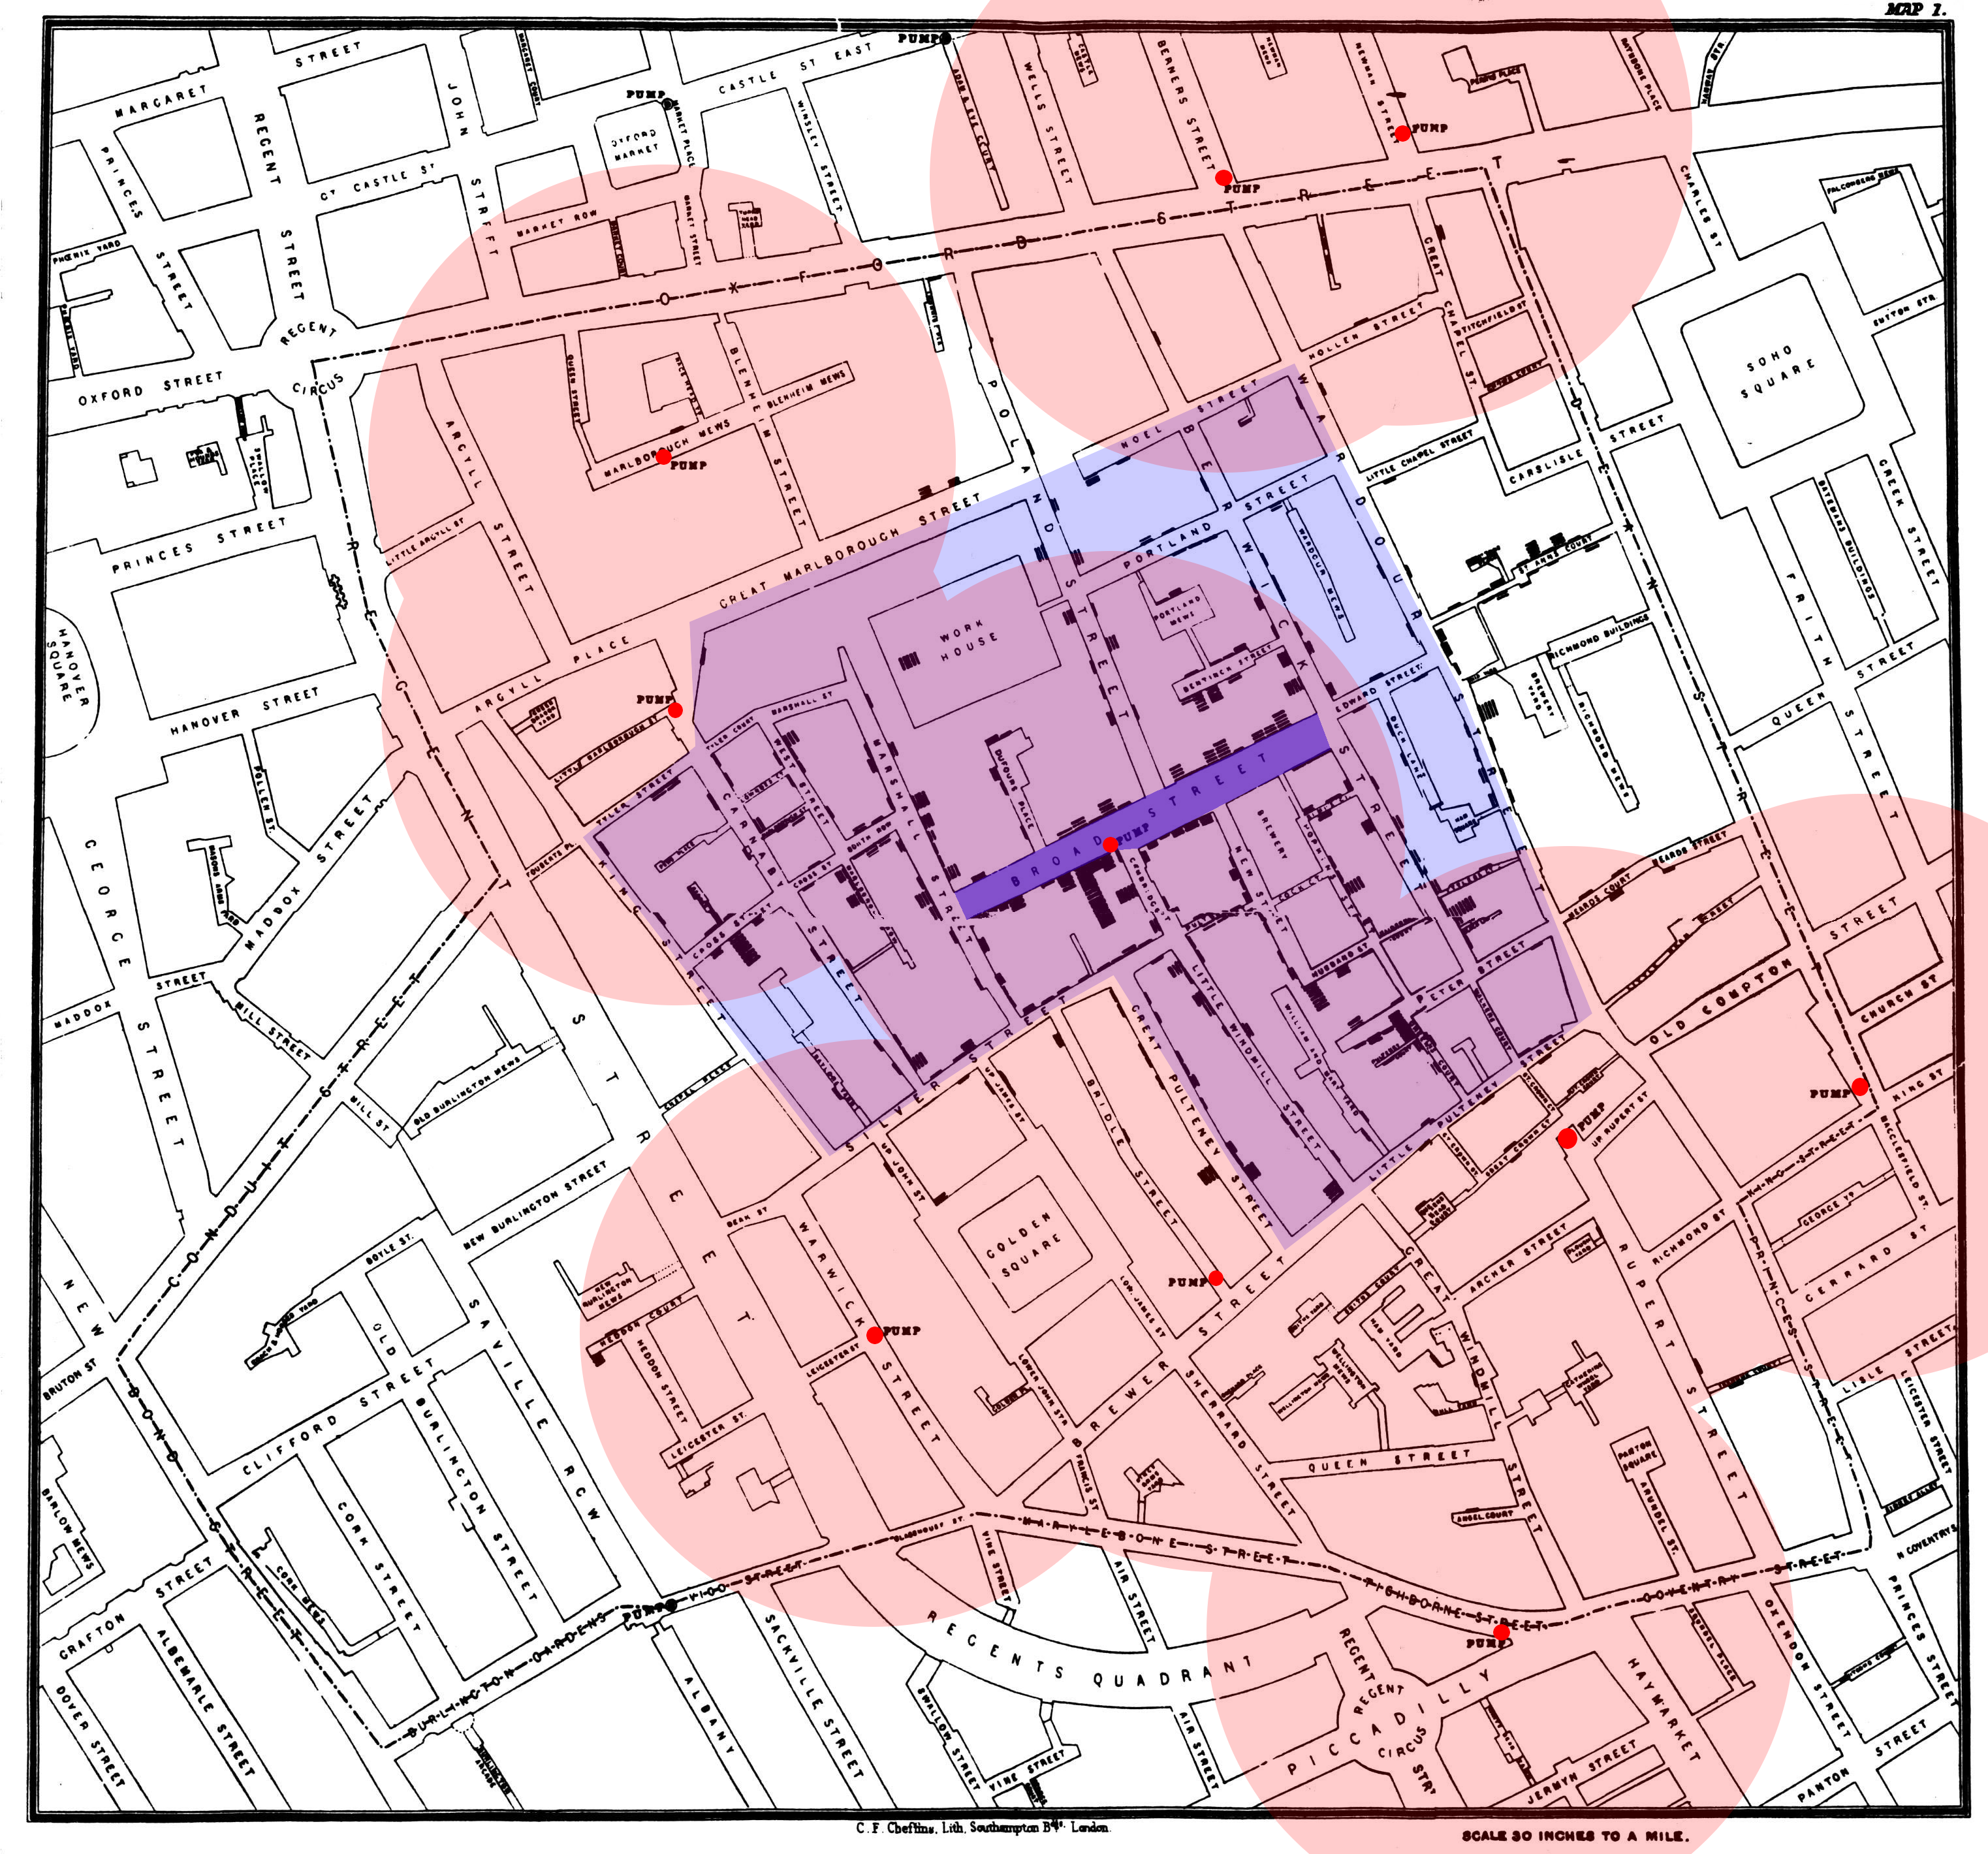
\includegraphics[height=.98\textheight]{images/broadstreet-4}}
\only<6>{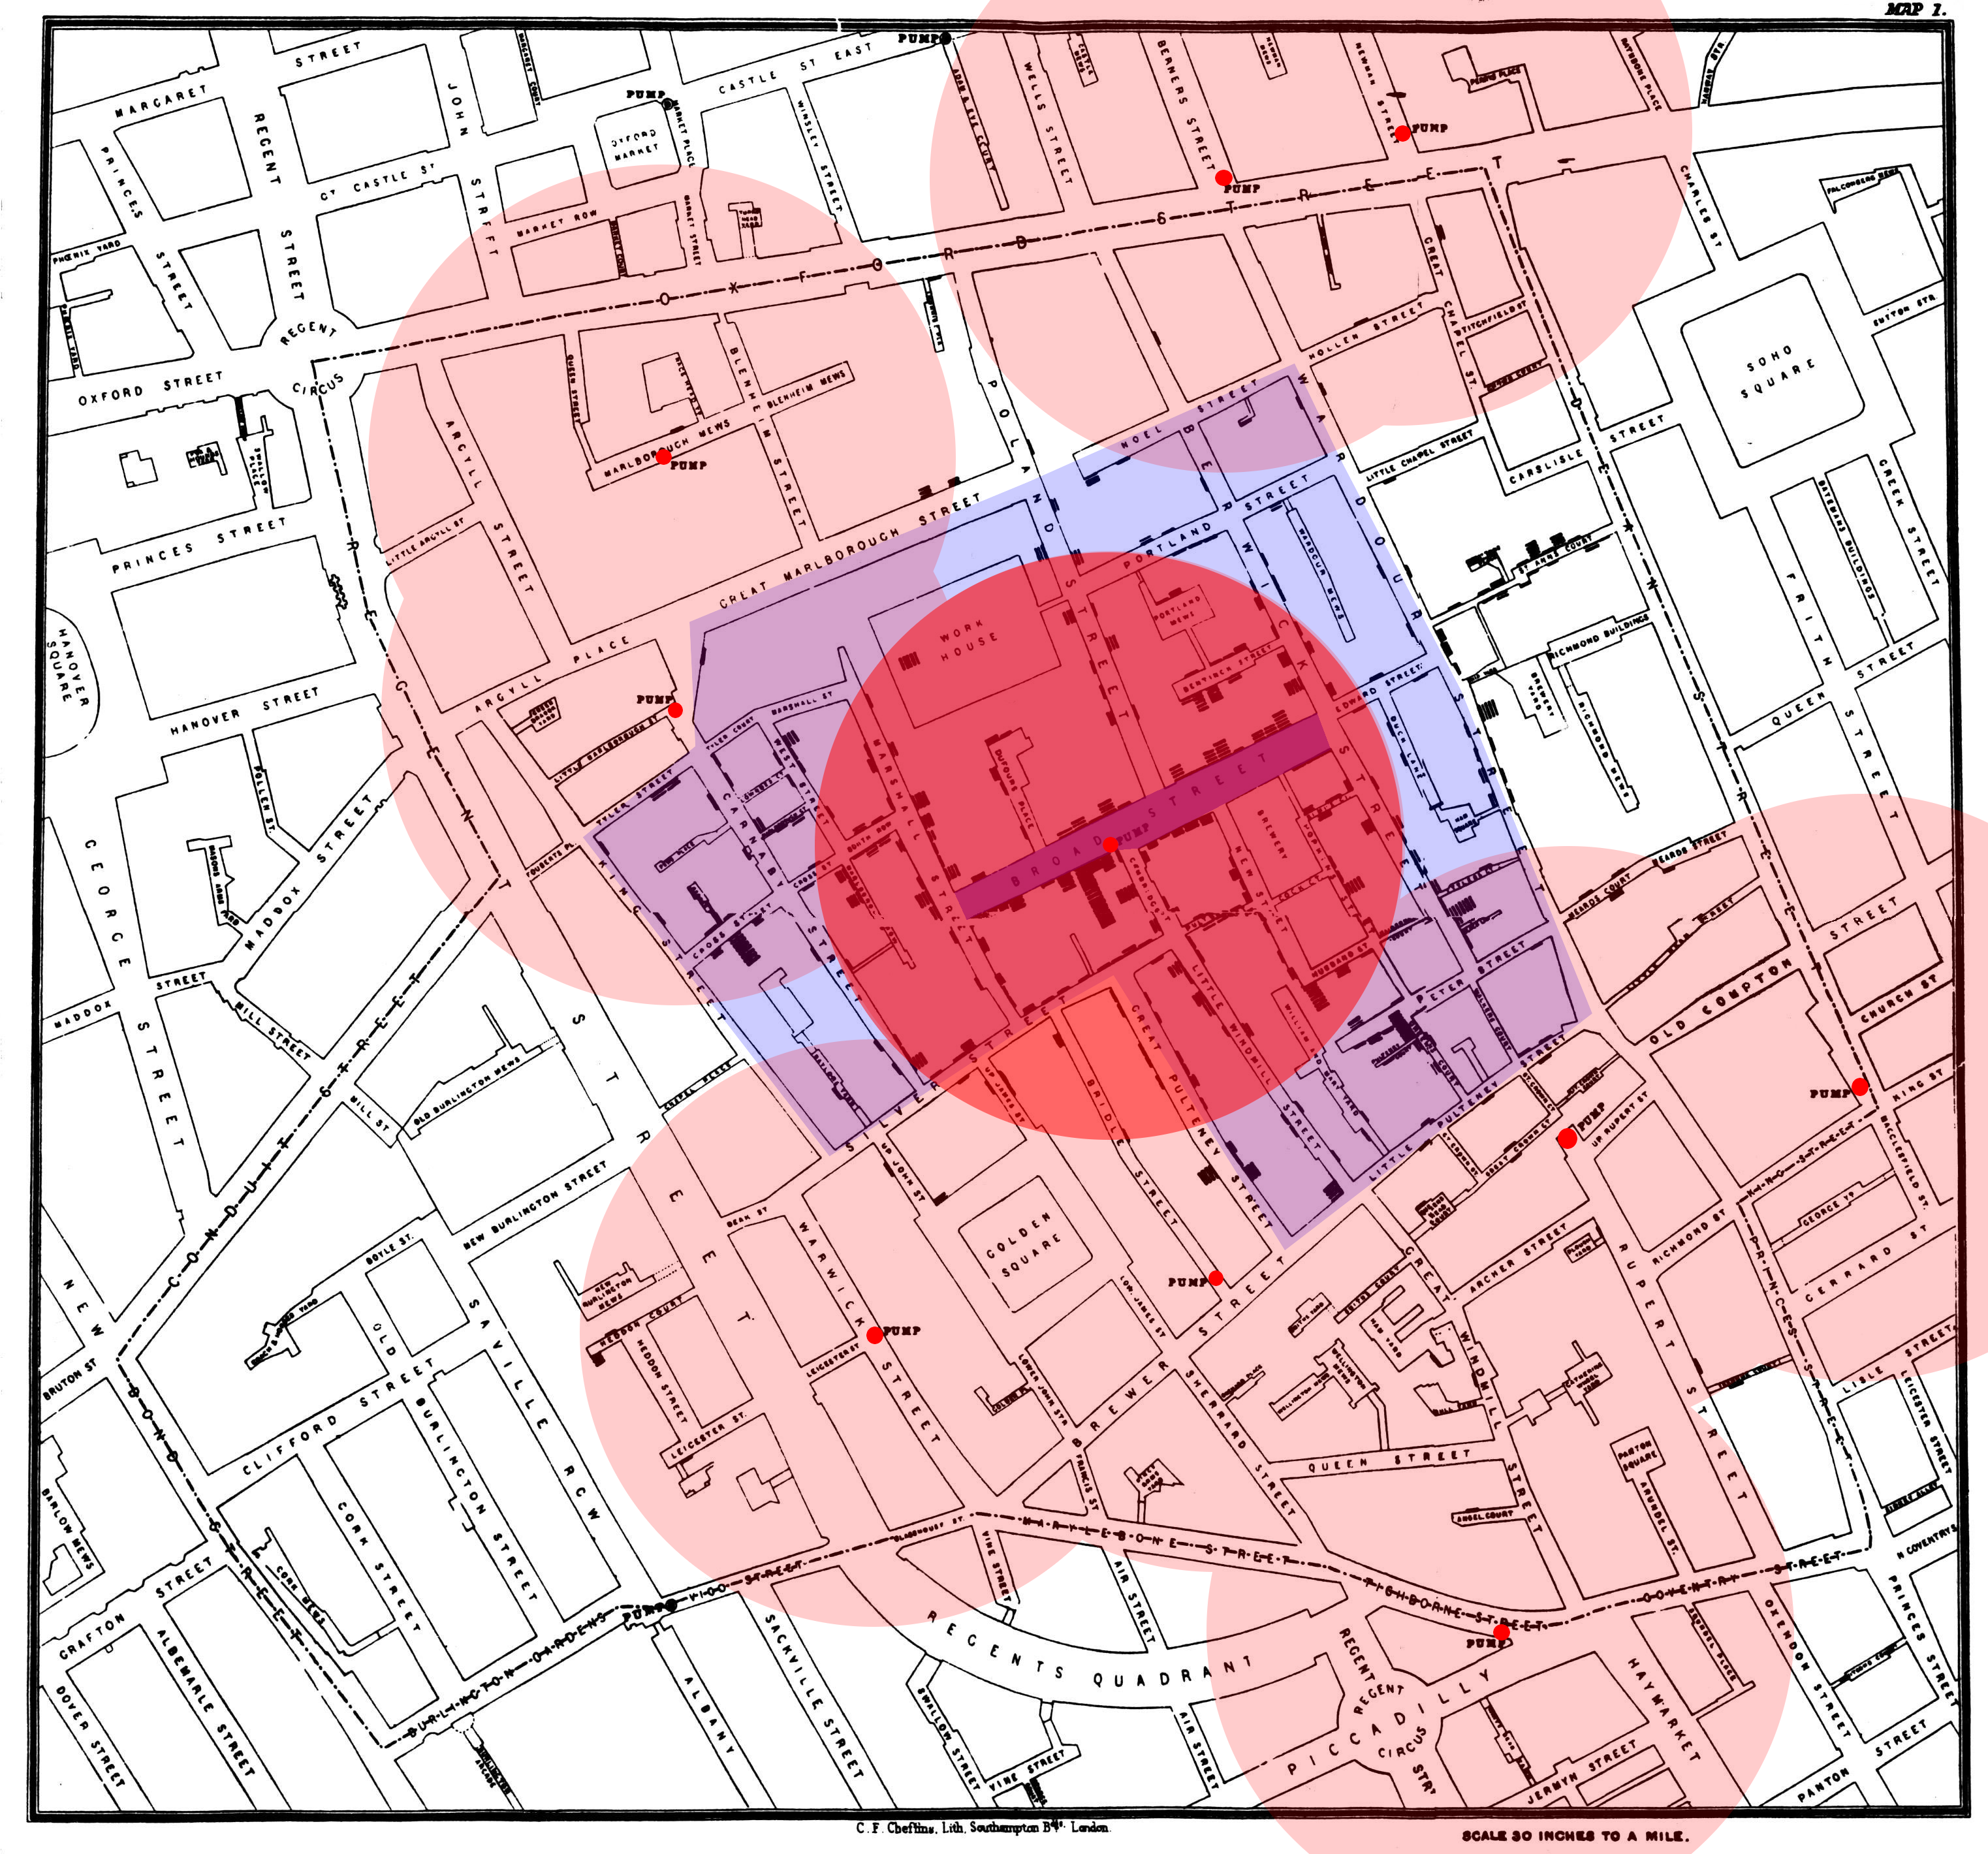
\includegraphics[height=.98\textheight]{images/broadstreet-5}}
\only<7>{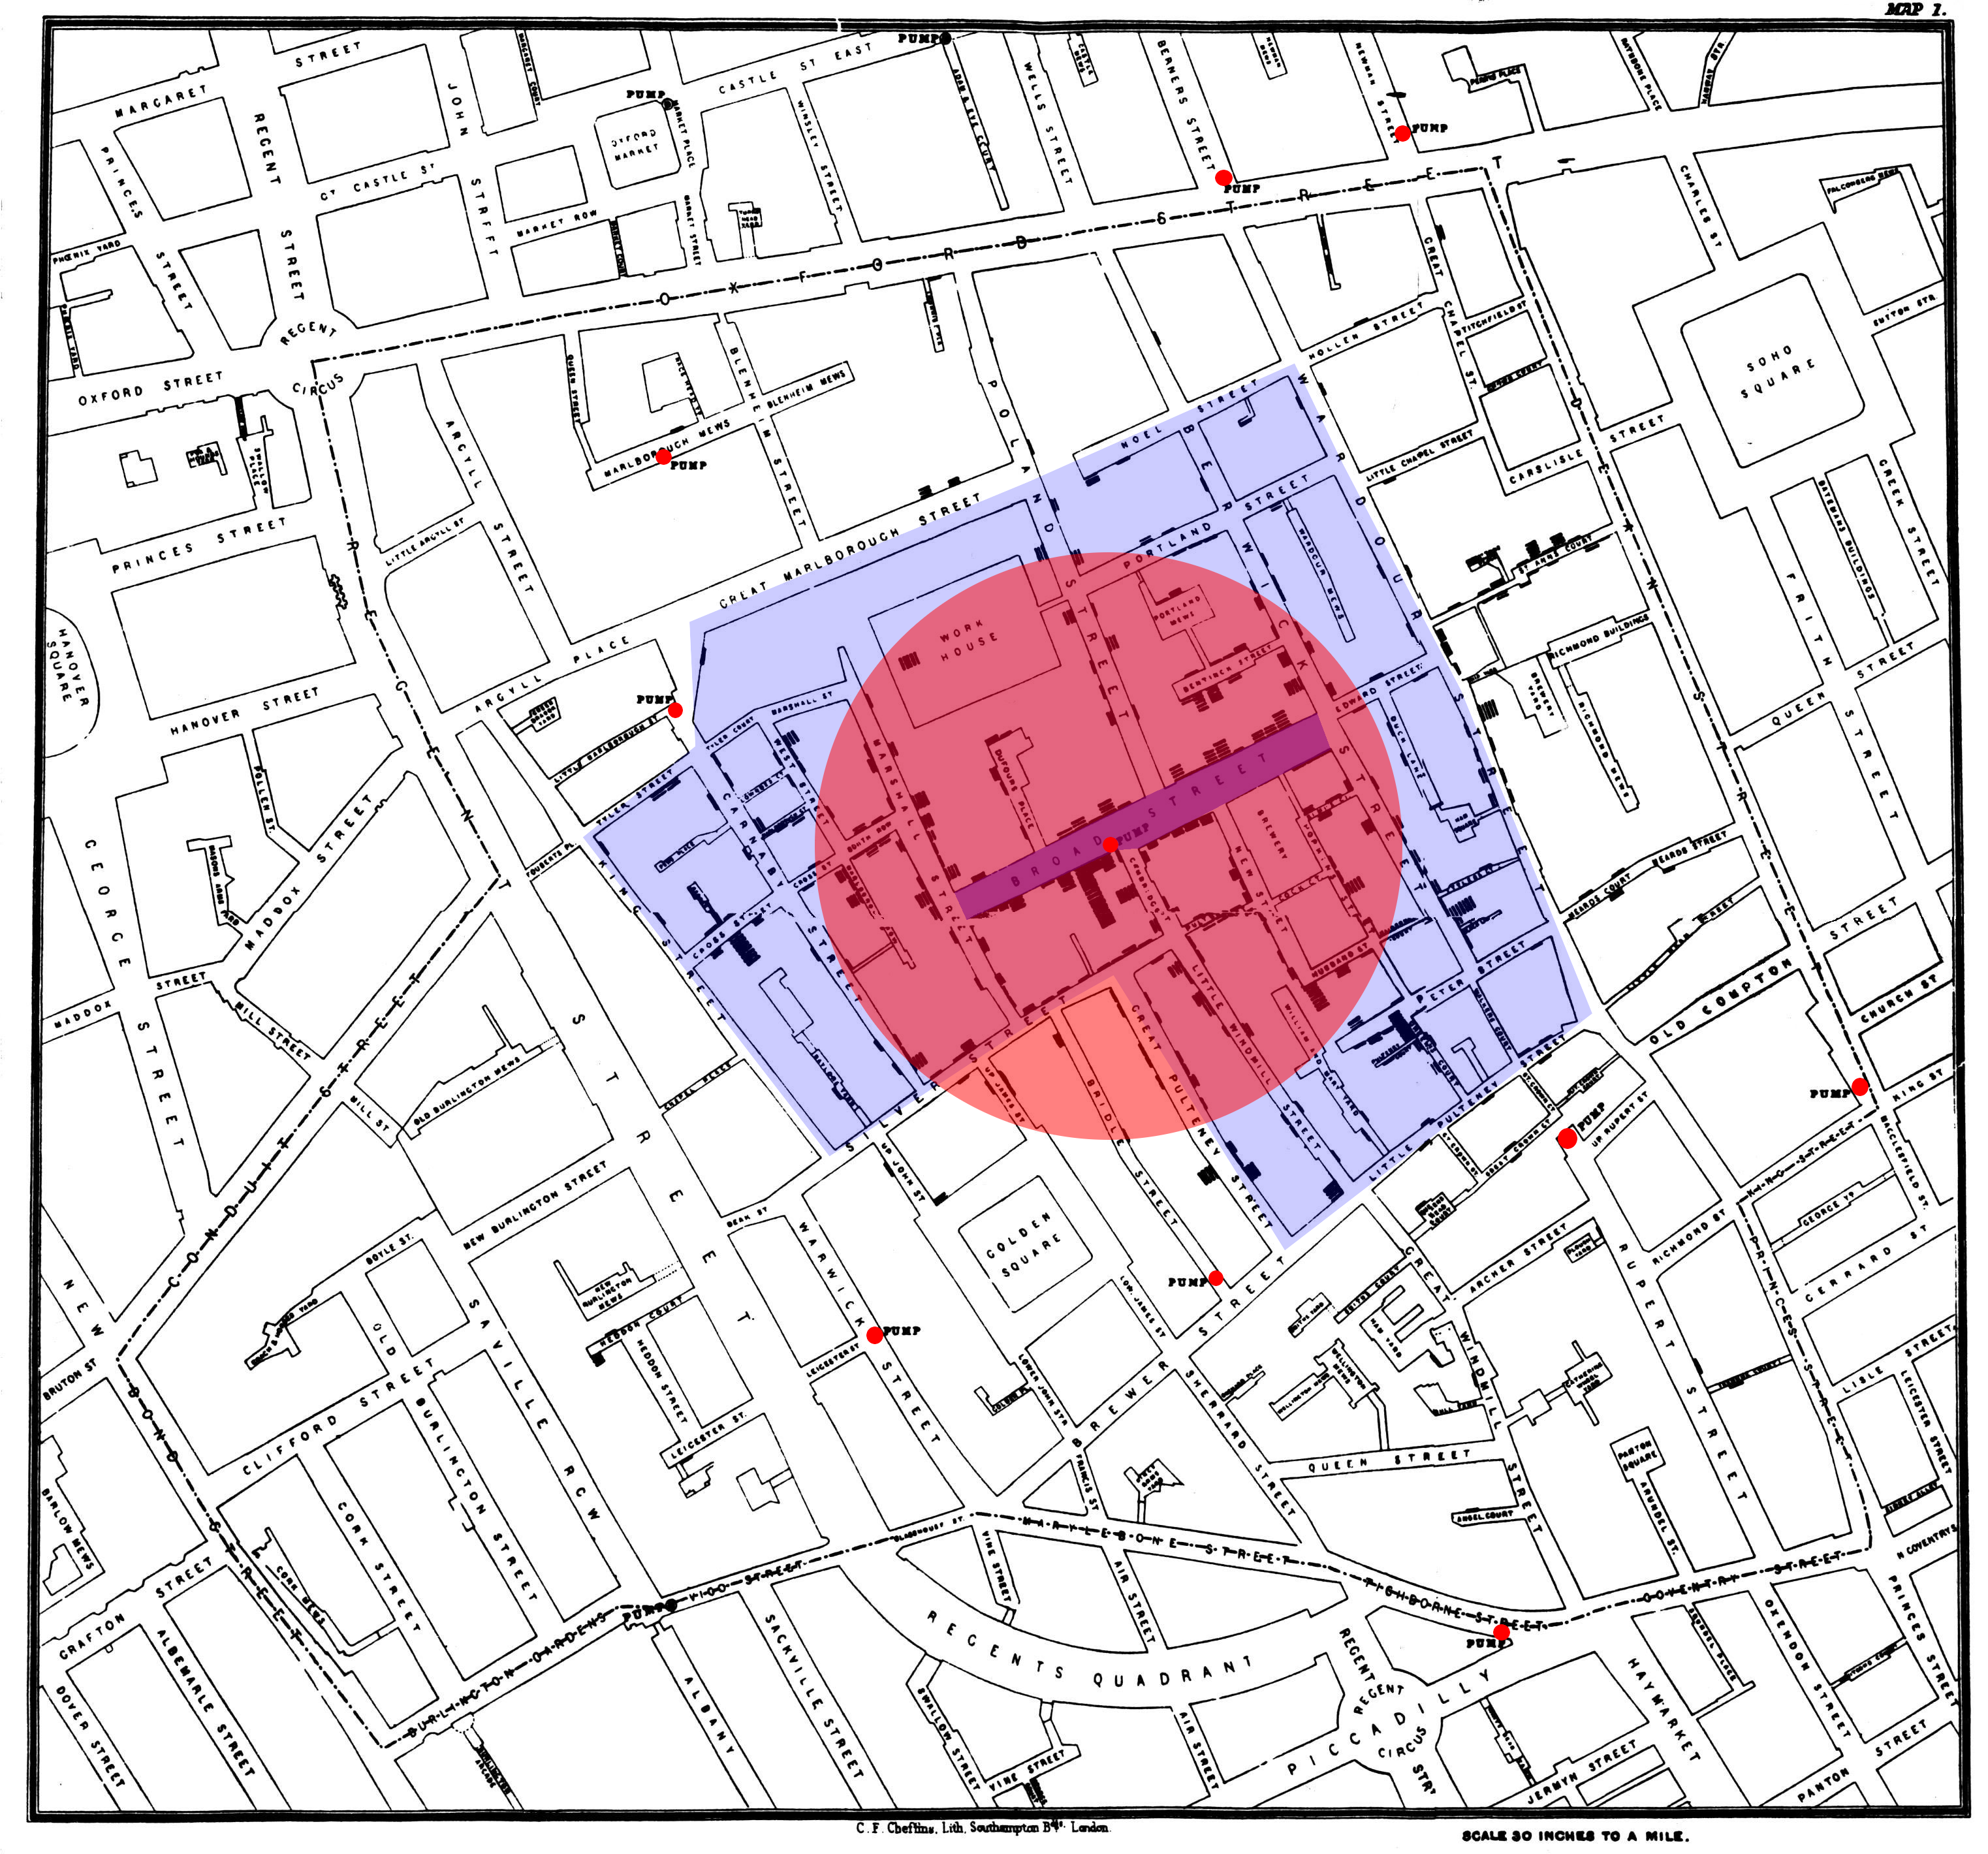
\includegraphics[height=.98\textheight]{images/broadstreet-6}}
\end{center}

{\footnotesize Image source: Public Domain from \href{https://en.wikipedia.org/wiki/File:Snow-cholera-map-1.jpg}{Wikipedia}}

}

\frame{

\frametitle{{\large Ex.: Gapminder Data}}

\begin{center}
\includegraphics[width=.9\textwidth]{images/gapminder}
\end{center}

}


% Brexit example?


\frame{}


\frame{

\frametitle{{\large ``Description''}}

\small 

\begin{itemize}\itemsep0.5em
\item ``Description'' is a label for many concepts
	\begin{itemize}
	\item Meaning is ambiguous
	\end{itemize}
\item<2-> Gerring describes many forms of description
	\begin{itemize}
	\item Summaries, associations
	\item Grouping/categorization (e.g., typologies)
	\item Accounts (e.g., biography, history)
	\end{itemize}
\item<3-> Toshkov has a different typology
	\begin{itemize}
	\item Multi-/single-case
	\item Multi-/uni-variate
	\end{itemize}
\end{itemize}

}

\frame{

\frametitle{Description $\equiv$ ``What?''}

\begin{itemize}
\item Common feature of descriptive research and descriptive research questions is a focus on \textit{what} questions

\item<2-> Examples
	\begin{itemize}
	\item<2-> What is this?
	\item<3-> What other things are (un)like this?
	\item<4-> What features does this have?
	\item<5-> What people, institutions, and ideas does this involve?
	\item<6-> Where is this? When is this?
	\item<7-> How much of this is there?
	\end{itemize}
\end{itemize}

}

% the answers to many of these questions are not DSOs


\frame{}


\frame{

\frametitle{Answering Descriptive RQs}

\begin{enumerate}\itemsep0.5em
\item Ask question
\item Decide what kind of evidence will answer that question
\item Gather evidence
\item Analyze evidence
\item Draw inferences and make claims
\item (Iterate)
\end{enumerate}

}

\frame{

\frametitle{Ex.: Broad Street Cholera}

\begin{enumerate}\itemsep0.25em
\item<2-> Who is getting cholera?
\item<3-> DSOs about who is sick (\& not sick)
\item<4-> Interview patients or use medical records
\item<5-> Examine associations between cholera and patient characteristics
\item<6-> Inference: Geographical clustering
\item<7-> Iterate: What is different about this geographical area?
\end{enumerate}

}



\frame{

\frametitle{{\large Common Methods of Descriptive Evidence Gathering}}

\begin{itemize}\itemsep0.25em
\item Direct observation
	\begin{itemize}
	\item Participant--observation
	\end{itemize}
\item Interviewing
	\begin{itemize}
	\item Surveys
	\item Elite interviews
	\item Focus groups
	\end{itemize}
\item Documentary analysis
	\begin{itemize}
	\item Archival research
	\item Text analysis
	\end{itemize}
\end{itemize}

}


\frame{

\frametitle{{\large Some RQ/Method Pairings}}

\begin{tabular}{p{2.5in}p{1.75in}}
RQ & Evidence \\ \midrule
What do people think? & Interviewing \\ \midrule
What happened? & Archival analysis \\ \midrule
How does this institution work? & ?? \\ \midrule
\end{tabular}

\only<2->{Yet, we often use non-obvious methods, and multiple methods.}
}


\frame{

\frametitle{Considerations}

\begin{itemize}
\item<2-> How do we decide what kind of evidence is appropriate?
\item<3-> How do we arbitrate between conflicting evidence?
\item<4-> How do we decide if evidence is ``true''?
\item<5-> How do we know when we have ``enough'' evidence?
\end{itemize}

}



\section{Texts as Sources}
\frame{\tableofcontents[currentsection]}


\frame{

\frametitle{What counts as text?}

\begin{itemize}\itemsep1em
\item Primary sources
	\begin{itemize}
	\item Raw, original evidence
	\end{itemize}
\item Secondary sources
	\begin{itemize}
	\item Interpretations of raw evidence
	\end{itemize}
\item Tertiary sources
	\begin{itemize}
	\item Compendia or indices of two other types of sources
	\end{itemize}
\end{itemize}

}
% brainstorm examples


\frame{

\frametitle{How do you use texts?}

\small

\begin{itemize}\itemsep0.75em
\item Think about your own experience reading, interpreting, and interacting with textual sources for academic purposes (e.g, for writing a term paper).
\item With the person sitting next to you, discuss:
	\begin{enumerate}
	\item The process by which you try to understand the meaning and content of texts
	\item How you choose texts to read
	\end{enumerate}
\end{itemize}

}

\frame{

\frametitle{Use of Texts}

\begin{itemize}\itemsep1em
\item<1-> Text as description
	\begin{itemize}
	\item Rely on text in lieu of direct observation
	\item What do we gain? What do we lose?
	\end{itemize}
\item<2-> Text as DSOs
	\begin{itemize}
	\item Treat texts as units (see MT Week 7)
	\end{itemize}
\end{itemize}


}

% texts in lieu of observation
% we cannot see everything ourselves, so we rely on evidence

\frame{

\frametitle{Challenges of Text}

\begin{enumerate}\itemsep1em
\item Source ``Quality''
\item Subjectivity and differing perspectives
\item Historiography
\item Selection and confirmation bias
\end{enumerate}

\onslide<2->{But these are really the challenges of \textit{any} research!}

}


% define historiography

% texts are subjective

% selection bias -> when do we stop looking for evidence?
% -> how do we know that we have all of the evidence?
% -> If we go looking for information about a case as something, do we miss evidence that sees that case as a case of something else?






\appendix
\frame{}

\end{document}
